\clearpage
\begin{proofbox}

	\textbf{\textcolor{CProof}{思路提示}}

先用能算出来的$2$的整数次幂找到规律，再用指数函数的单调性证明规律对所有正真数都成立；最后逐个检查“过定点”和“两种对称”对应的坐标。

	\medskip
	\textbf{\textcolor{CProof}{方法一（最低门槛：把指数表倒过来看）}}
\begin{center}\begin{tikzpicture}[font=\small,>=stealth,line join=round]
\draw[gray!40,rounded corners=3pt] (0,0) rectangle (14.2,9.1);\node at (7.1,8.5) {方法一：2的一次方是2，反过来问得到对数};
\begin{scope}[shift={(2.6,3.1)},x=.94cm,y=.94cm]\draw[->,gray] (-1.5,0)--(4.4,0) node[right]{$x$};\draw[->,gray] (0,-1.5)--(0,4.4) node[above]{$y$};\draw[gray,dashed] (-1.3,-1.3)--(4,4);\draw[blue!75!black,thick,domain=.42:4.1,samples=160] plot(\x,{ln(\x)/ln(2)});\draw[violet,thick,dashed,domain=-1.3:2.04,samples=160] plot(\x,{pow(2,\x)});\fill[violet] (1,2) circle(2pt);\fill[blue!75!black] (2,1) circle(2pt);\draw[gray,densely dotted] (1,2)--(2,1);\node[below right=4pt] at (3.2,3.2){$y=x$};\end{scope}\node[anchor=west,text width=5cm,align=left] at (8.5,4.5) {紫虚线：$y=2^x$\\[8pt]蓝实线：$y=\log_2x$\\[8pt]$(1,2)\leftrightarrow(2,1)$\\[8pt]横、纵坐标交换\\[8pt]一般：$(u,v)\leftrightarrow(v,u)$};
\node[text width=12.6cm,align=center] at (7.1,.65) {两轴单位相同；(1,2)与(2,1)交换坐标。几个数字帮助发现规律，不能代替一般证明。};
\end{tikzpicture}\end{center}



先列出$2^{-2}=\tfrac14$、$2^{-1}=\tfrac12$、$2^0=1$、$2^1=2$、$2^2=4$；倒过来就是
\[
\log_2\tfrac14=-2,\quad \log_2\tfrac12=-1,\quad
\log_2 1=0,\quad \log_2 2=1,\quad\log_2 4=2.
\]
如果底数换成$\tfrac12$，相同五个真数对应的指数顺序就反过来。这能直观\textbf{发现}增减规律，但只列五个数还不能替代对所有正数的证明；下一种方法将补上这一点。

\begin{center}
\begin{tikzpicture}[x=1.05cm,y=0.68cm,>=stealth]
 \foreach \xx/\s in {0/{1/4},1/{1/2},2/1,3/2,4/4}{
   \draw[fill=blue!7,draw=blue!40,rounded corners=1.2pt] (\xx-0.36,0.12) rectangle (\xx+0.36,0.68);
   \node at (\xx,0.4) {\small $\s$};
 }
 \draw[->,thick,blue!75!black] (-0.3,-0.12)--(4.4,-0.12);
 \node[left] at (-0.4,0.4) {\small 真数};
 \node[below] at (2,-0.18) {\small 从左到右真数变大；底数$2$的指数$-2,-1,0,1,2$也变大};
\end{tikzpicture}
\end{center}

\medskip

\end{proofbox}
\clearpage
\begin{proofbox}
\textbf{\textcolor{CProof}{方法二（高中常规：用指数函数证明所有情况）}}
\begin{center}\begin{tikzpicture}[font=\small,>=stealth,line join=round]
\draw[gray!40,rounded corners=3pt] (0,0) rectangle (14.2,8.8);\node at (7.1,8.200000000000001) {方法二：固定两个输出，反过来寻找所需的指数};
\node at (3.1500000000000004,7.3) {$a=2$};\begin{scope}[shift={(3.1500000000000004,3.3000000000000003)},x=1.53125cm,y=1.0000000000000002cm]\draw[->,gray] (-1.6,0)--(1.6,0) node[right]{指数};\draw[->,gray] (0,-0.3)--(0,3) node[above]{输出};\draw[blue!75!black,thick,solid,domain=-1.3:1.3,samples=180] plot(\x,{pow(2,\x)});\fill[orange!85!black] (-1,0.5) circle(2pt);\fill[orange!85!black] (1,2) circle(2pt);\draw[gray!35,densely dotted] (-1,0)--(-1,-0.3);\node[below=3pt] at (-1,-0.3){$-1$};\draw[gray!35,densely dotted] (1,0)--(1,-0.3);\node[below=3pt] at (1,-0.3){$1$};\draw[gray,densely dotted] (-1.4,.5)--(1.4,.5);\draw[gray,densely dotted] (-1.4,2)--(1.4,2);\end{scope}\node[align=center,text width=5.8cm] at (3.1500000000000004,1.7) {输出$\frac12<2$\\对应指数$-1<1$};\node at (9.95,7.3) {$a=\frac12$};\begin{scope}[shift={(9.95,3.3000000000000003)},x=1.53125cm,y=1.0000000000000002cm]\draw[->,gray] (-1.6,0)--(1.6,0) node[right]{指数};\draw[->,gray] (0,-0.3)--(0,3) node[above]{输出};\draw[orange!85!black,thick,solid,domain=-1.3:1.3,samples=180] plot(\x,{pow(0.5,\x)});\fill[orange!85!black] (-1,2.0) circle(2pt);\fill[orange!85!black] (1,0.5) circle(2pt);\draw[gray!35,densely dotted] (-1,0)--(-1,-0.3);\node[below=3pt] at (-1,-0.3){$-1$};\draw[gray!35,densely dotted] (1,0)--(1,-0.3);\node[below=3pt] at (1,-0.3){$1$};\draw[gray,densely dotted] (-1.4,.5)--(1.4,.5);\draw[gray,densely dotted] (-1.4,2)--(1.4,2);\end{scope}\node[align=center,text width=5.8cm] at (9.95,1.7) {输出$\frac12<2$\\对应指数$1>-1$};
\node[text width=12.6cm,align=center] at (7.1,.65) {两图同尺度；横轴为指数，纵轴为输出。大底数保序，小底数反序。};
\end{tikzpicture}\end{center}



\textbf{先证定义域、值域和定点：}由$y=\log_a x\Longleftrightarrow x=a^y$，每个$a^y$都大于$0$，所以$x>0$；任意实数$y$都能使$x=a^y>0$，所以值域为$\mathbb R$。又因$a^0=1$，故$\log_a1=0$，定点$(1,0)$。

\medskip
\textbf{\textcolor{CProof}{正式推导}}
	\begin{description}[style=nextline, leftmargin=2.8em, labelsep=0.5em, itemsep=0.55em]
		\item[\textbf{步骤一（化指为对）：}] 任取$0<x_1<x_2$，设$y_1=\log_a x_1$，$y_2=\log_a x_2$，由对数定义得
			\[
				a^{y_1}=x_1,
				\qquad
				a^{y_2}=x_2.
			\]
			\par\textbf{理由：} 对数定义$a^{\log_a N}=N$。

		\item[\textbf{步骤二（底数$a>1$时单调性）：}] 当$a>1$时，指数函数$y=a^x$在$\mathbb{R}$上单调递增。由$x_1<x_2$得$a^{y_1}<a^{y_2}$，再由指数递增性得$y_1<y_2$，即$\log_a x_1<\log_a x_2$。
			\par\textbf{理由：} 指数函数单调递增，底数大于1时$a^{u}<a^{v}\Leftrightarrow u<v$。

		\item[\textbf{步骤三（底数$0<a<1$时单调性）：}] 当$0<a<1$时，指数函数$y=a^x$在$\mathbb{R}$上单调递减。由$x_1<x_2$得$a^{y_1}<a^{y_2}$，由指数递减性得$y_1>y_2$，即$\log_a x_1>\log_a x_2$。
			\par\textbf{理由：} 指数函数单调递减，$a^{u}<a^{v}\Leftrightarrow u>v$。

		\item[\textbf{步骤四（符号判定）：}] 由于$f(1)=\log_a 1=0$，结合单调性：
			\begin{itemize}
			\item 若$a>1$，函数递增，则$x>1$时$f(x)>f(1)=0$；$0<x<1$时$f(x)<f(1)=0$。
			\item 若$0<a<1$，函数递减，则$x>1$时$f(x)<f(1)=0$；$0<x<1$时$f(x)>f(1)=0$。
		\end{itemize}
			\par\textbf{理由：} 单调函数的值符号由自变量与$1$的相对大小及单调性共同决定。
	\end{description}

	\medskip
	
\begin{center}
\begin{tikzpicture}[x=1cm,y=0.66cm,>=stealth]
 \draw[->,gray] (-0.2,0)--(3.55,0) node[right] {$x$};
 \draw[->,gray] (0,-1.4)--(0,1.9) node[above] {$y$};
 \draw[thick,blue!75!black,domain=0.4:3.2,samples=65] plot (\x,{ln(\x)/ln(2)});
 \fill[blue!75!black] (0.5,-1) circle(1.6pt) node[below right] {\small $(\tfrac12,-1)$};
 \fill[blue!75!black] (2,1) circle(1.6pt) node[above left] {\small $(2,1)$};
 \draw[->,blue!65] (1.05,-0.9)--(1.85,0.75);
\end{tikzpicture}
\par\small 严格证明说明：这种向右升高不是只在图中的几个点成立。
\end{center}

\medskip

\end{proofbox}
\clearpage
\begin{proofbox}
\textbf{\textcolor{CProof}{方法三（坐标验算：两种对称究竟怎样证明）}}
\begin{center}\begin{tikzpicture}[font=\small,>=stealth,line join=round]
\draw[gray!40,rounded corners=3pt] (0,0) rectangle (14.2,8.3);\node at (7.1,7.700000000000001) {方法三的第一种对称：同一真数，函数值取相反数};
\begin{scope}[shift={(1.589795918367347,3.9499999999999997)},x=1.2244897959183672cm,y=0.7666666666666666cm]\draw[->,gray] (-0.4,0)--(4.5,0) node[right]{$x$};\draw[->,gray] (0,-3)--(0,3) node[above]{$y$};\draw[blue!75!black,thick,solid,domain=0.18:4,samples=180] plot(\x,{ln(\x)/ln(2)});\draw[orange!85!black,thick,dashed,domain=0.18:4,samples=180] plot(\x,{ln(\x)/ln(0.5)});\fill[orange!85!black] (2,1) circle(2.2pt);\fill[orange!85!black] (2,-1) circle(2.2pt);\fill[orange!85!black] (1,0) circle(2.2pt);\draw[gray,dashed] (2,-1)--(2,1);\draw[gray!35,densely dotted] (1,0)--(1,-3);\node[below=3pt] at (1,-3){$1$};\draw[gray!35,densely dotted] (2,0)--(2,-3);\node[below=3pt] at (2,-3){$2$};\draw[gray!35,densely dotted] (4,0)--(4,-3);\node[below=3pt] at (4,-3){$4$};\end{scope}\node[anchor=west,align=left,text width=5.0cm] at (8.4,4.0) {$\log_{1/a}x=-\log_ax$\\[10pt]$(2,1)\leftrightarrow(2,-1)$\\[10pt]横坐标相同\\[10pt]纵坐标互为相反数\\[10pt]对称轴为$x$轴};
\node[text width=12.6cm,align=center] at (7.1,.65) {对称时改变的是纵坐标；一般点(x,t)对应(x,-t)，x仍然大于0。};
\end{tikzpicture}\end{center}



\textbf{第一种，两个底数互为倒数的对数函数。}任取$x>0$，设$t=\log_a x$，于是$a^t=x$。因为
\[
 \left(\frac1a\right)^{-t}=a^t=x,
\]
所以$\log_{1/a}x=-t=-\log_a x$。第一条图像上每个点$(x,t)$，在第二条图像中都有点$(x,-t)$；\textbf{横坐标不变、纵坐标变相反数}，因此关于$x$轴对称。

\begin{center}
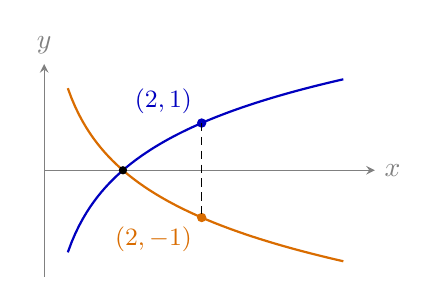
\begin{tikzpicture}[x=1.0cm,y=0.6cm,>=stealth]
 \draw[->,gray] (0,0)--(4.2,0) node[right] {$x$};
 \draw[->,gray] (0,-2.25)--(0,2.25) node[above] {$y$};
 \draw[blue!75!black,thick,domain=0.3:3.8,samples=75] plot(\x,{ln(\x)/ln(2)});
 \draw[orange!85!black,thick,domain=0.3:3.8,samples=75] plot(\x,{-ln(\x)/ln(2)});
 \fill[blue!75!black] (2,1) circle (1.7pt) node[above left] {\small $(2,1)$};
 \fill[orange!85!black] (2,-1) circle (1.7pt) node[below left] {\small $(2,-1)$};
 \draw[densely dashed] (2,1)--(2,-1);
 \fill (1,0) circle(1.5pt);
\end{tikzpicture}
\par\small 上下两点横坐标相同、纵坐标互为相反数，因此关于$x$轴对称。
\end{center}


\end{proofbox}
\clearpage
\begin{proofbox}
\textbf{第二种，指数函数与对数函数。}
\begin{center}\begin{tikzpicture}[font=\small,>=stealth,line join=round]
\draw[gray!40,rounded corners=3pt] (0,0) rectangle (14.2,9.1);\node at (7.1,8.5) {方法三的第二种对称：交换坐标，沿y=x翻折};
\begin{scope}[shift={(2.6,3.1)},x=.94cm,y=.94cm]\draw[->,gray] (-1.5,0)--(4.4,0) node[right]{$x$};\draw[->,gray] (0,-1.5)--(0,4.4) node[above]{$y$};\draw[gray,dashed] (-1.3,-1.3)--(4,4);\draw[blue!75!black,thick,domain=.42:4.1,samples=160] plot(\x,{ln(\x)/ln(2)});\draw[violet,thick,dashed,domain=-1.3:2.04,samples=160] plot(\x,{pow(2,\x)});\fill[violet] (0,1) circle(2pt);\fill[blue!75!black] (1,0) circle(2pt);\draw[gray,densely dotted] (0,1)--(1,0);\node[below right=4pt] at (3.2,3.2){$y=x$};\end{scope}\node[anchor=west,text width=5cm,align=left] at (8.5,4.5) {紫虚线：$y=2^x$\\[8pt]蓝实线：$y=\log_2x$\\[8pt]$(0,1)\leftrightarrow(1,0)$\\[8pt]横、纵坐标交换\\[8pt]一般：$(u,v)\leftrightarrow(v,u)$};
\node[text width=12.6cm,align=center] at (7.1,.65) {指数图像上的(0,1)交换成对数图像上的(1,0)，不是把原来的点原封不动搬过去。};
\end{tikzpicture}\end{center}

若指数图像上有一点$(u,v)$，则$v=a^u$。将等式倒过来写为$u=\log_a v$（此时$v>0$），可知对数图像上有一点$(v,u)$。坐标互换对应关于$y=x$翻折。特别地：指数图像上的$(0,1)$，换过去是对数图像上的$(1,0)$；\textbf{绝不能把$(0,1)$直接当成对数图像上的点}，因为对数不能取$x=0$。

\medskip
\textbf{\textcolor{CProof}{结论回扣}}

	“表格”负责帮助理解，“指数单调性”负责严格证明，“坐标交换和取相反数”负责证明对称。单调性由底数决定，但函数值的正负还要看真数在$1$的哪一侧。

\end{proofbox}
